\section{Performance Evaluation, Results, Discussion}

\textit{owners: Evan: graphs, All: interpretation (2.75 pages)}

\begin{itemize}
\item Platform Descriptions
\begin{itemize}
  \item EC2

  \item XC40
  \item Experimental Cray Cluster (EXP\_CC)
\end{itemize}

\item CX Spark Implementation Phase Descriptions
 \begin{enumerate}
      \item Load Matrix Metadata
      \item Load Matrix
      \item Iterations
      \item Postprocessing/Collect
 \end{enumerate}

 \item Dataset Sizes
 \begin{itemize}
  \item 100GB

  \item 1 TB

\end{itemize}
 \end{itemize}




  \subsection{Single Node Scaling Table}

  \begin{center}
  \begin{tabular}{ |c|c|c| } 
  \hline
  Single Node Optimization & Overall Speedup\\
  \hline
  Original Implementation & 1.0  \\
  Multi-Core Synchronization & 6.5 \\
  Cache Blocking & 15.6 \\
  SIMD & 39.7 \\
  \hline

  \end{tabular}
  \end{center}
  \textbf{Table 1: Single node optimizations to the CX C implementation and the subsequent speedup each additional optimization provides}
 



  \subsection{Scaling}
    \begin{figure} [H]
    \begin{centering}
    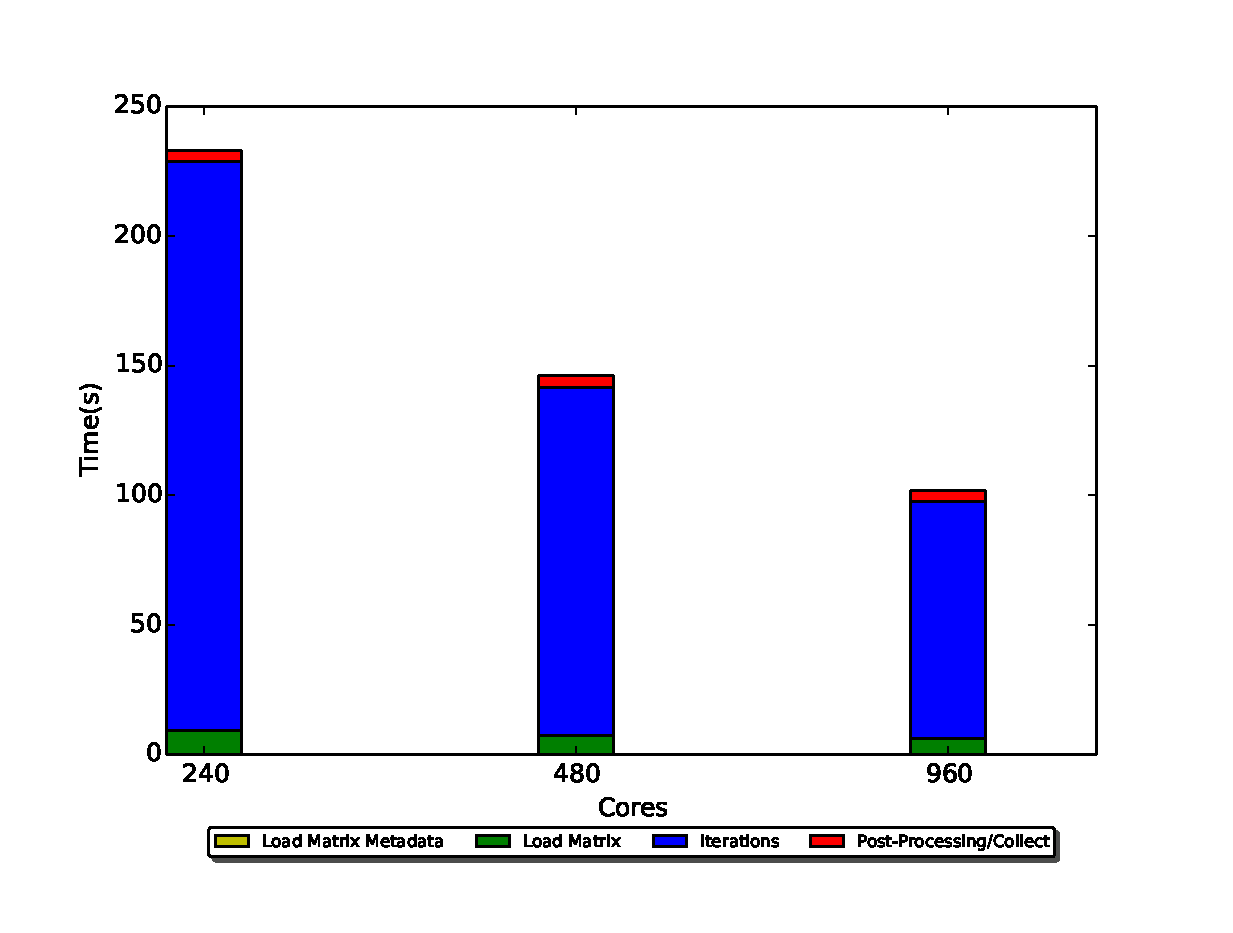
\includegraphics[scale=0.4]{images/CX_Strong_Scaling_32_Partitions_default.eps}
    \end{centering}
    \caption{ Strong scaling for the 4 phases of CX on an XC40 for 100GB dataset at rank 32 and default partitioning as concurrency is increased.} 
    \end{figure} 


  \subsection{Dataset Size Scaling Across Platforms}
    
    \begin{figure} [H]
    \begin{centering}
    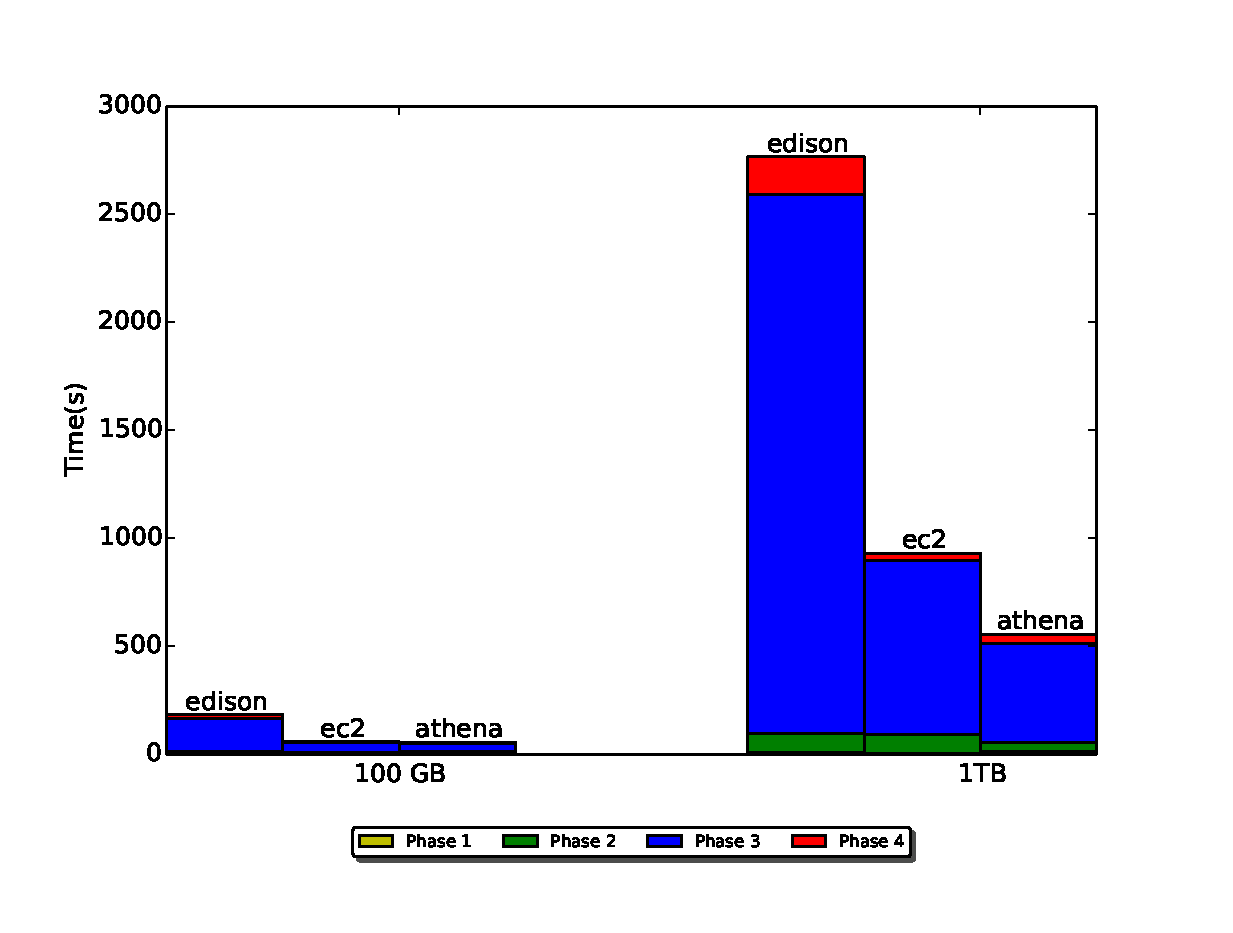
\includegraphics[scale=0.4]{images/CX_Size_Scaling_Rank_16_Partitions_default.eps}
    \end{centering}
    \caption{ Run times for the various stages of computation for CX for two different dataset sizes for the three platforms using rank 16 and default partitioning for the given platform} 
    \end{figure}
  

  \subsection{Comparison of CX, PCA, RPCA quantitatively (Alex will work on this)? }
    \begin{itemize}
      \item (for 100GB sized dataset on EC2)
      \item runtime vs. accuracy?
      \item show distinction b/w cx, pca
      \item alex will take ownership
    \end{itemize}

  \subsection{Science plot for PCA, CX (Jiyan and Oliver will produce this)}

